\section{The ForeC Language}
\label{sec:forecLanguage}

%-----------------------------------------------------------------------------

\subsection{The Synchronous Approach}
Synchronous languages are based on the synchronous hypothesis~\cite{timed_synchronous_survey},
which states that a system reacts instantaneously to new environmental
inputs. Thus, the synchronous hypothesis assumes that the system 
executes infinitely fast, in zero time. This separates the physical 
time of the environment from the execution time of the implemented system. 
Figure~\ref{fig:synchronous_moc} depicts a synchronous 
program, defined as a set of concurrent threads, interacting with the 
environment. Synchronous programs are driven by a hypothetical (logical)
\emph{global clock} that triggers the execution of the program. The speed 
of the global clock is determined by the system's specifications. At each
global tick, the threads sample the environment, perform their computations,
and then emit their results to the environment. When a thread completes 
its computation, we say that the thread has completed its \emph{local tick}.
When all threads have completed their local tick, we say that the program
has completed its \emph{global tick}.
Concurrent threads can communicate with each other (dashed 
arrows in Figure~\ref{fig:synchronous_moc}) during their
computation. The communication is instantaneous due to 
the synchronous hypothesis.   
The separation of physical and execution time simplifies 
the language semantics and enables formal verification. Once the 
system is implemented, it is necessary to verify the synchronous 
hypothesis. That is, the Worst-Case Execution Time (WCET) of each 
global tick must not exceed the specified period (in physical time) 
of the global clock.

\begin{figure}
	\centering
	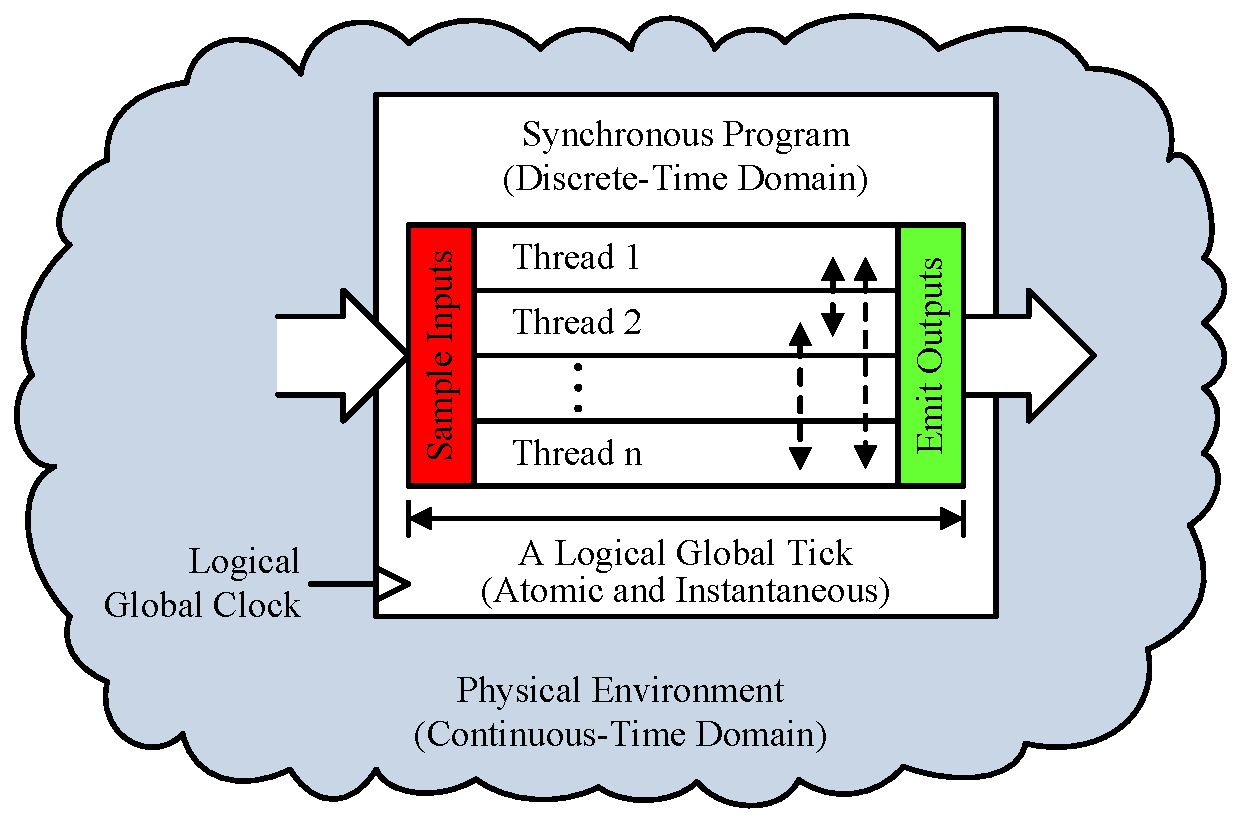
\includegraphics[width=0.6\columnwidth]{synchronous_moc}	

	\caption{Synchronous model of computation.}
	\label{fig:synchronous_moc}
\end{figure}

ForeC extends the C language with synchronous constructs to 
enable the deterministic parallel programming of multicores.
Extending C with synchronous constructs is not new, as the 
following languages demonstrate: Esterel-C Language (ECL~\cite{timed_ecl}), 
\synchronousc{} (SC~\cite{timed_synccharts_c_proposal}), Reactive 
Shared Variables~\cite{timed_reactivec_shared_variables}, 
and \pretc{}~\cite{pret_pretc}. The ECL compiler splits an 
ECL program into an Esterel and a C program. The Esterel program
is compiled in the traditional manner~\cite{timed_compiling_esterel}, 
where the concurrency is compiled away and, therefore, unsuitable for multicore execution.
The inherent sequential execution semantics of SC, Reactive C 
and \pretc{} renders them unsuitable for multicore execution. In
contrast, the semantics of ForeC is designed for parallel 
execution and does not impose
a scheduling order on parallel threads. Parallel threads can
be scheduled in an arbitrary order without altering the program's 
behaviour and allows the implementations to balance high execution 
performance against time-predictable execution. This scheduling 
independence is maintained even when threads communicate using 
shared variables. The remainder of this section details the 
syntax and semantics of the ForeC synchronous constructs.


%-----------------------------------------------------------------------------

\subsection{The ForeC Language Constructs}
ForeC extends C with additional instructions and type-qualifiers.
Figure~\ref{fig:forec_syntax} gives the extended syntax and 
Table~\ref{table:forec_semantics} summarises their semantics.  
A ForeC instruction can be either a classical C instruction or 
block within ``\verb${$'' and ``\verb$}$'' (\emph{c\_inst}), a
barrier synchronisation (\verb$pause$), an encapsulated fork/join
(\verb$par$), or hierarchical preemption (\verb$abort$). ForeC
variables are declared like in C with a type and type qualifier, 
which can be a C type qualifier (\emph{c\_tq}), a qualifier to 
denote variables that are updated by the environment (\verb$input$), a 
qualifier to denote variables that are emitted to the
environment (\verb$output$), or a qualifier to denote variables
that are shared between threads (\verb$shared$). In a variable 
declaration, the ForeC type qualifiers must precede the C type 
qualifiers. We continue by describing each ForeC construct in detail.

\begin{figure}[t]
	\centering

	\renewcommand{\arraystretch}{1.25}
	\begin{tabular}{l r l}
		Instructions:		& \emph{inst} & ::= \emph{c\_inst}																\\
							&			& ~~~| \verb$pause$ | \verb$par($\emph{inst}(,~\emph{inst})*\verb$)$				\\
							&			& ~~~| \verb$weak$?~\verb$abort$~\emph{inst}~\verb$when immediate$?~(\expression{})	\\
																															\\
		Type-Qualifiers:	& \emph{tq}	& ::= \emph{c\_tq}																	\\
							&			& ~~~| \verb$input$ | \verb$output$ | \verb$shared$
	\end{tabular}
	
	\caption{The syntactic extensions to C.}
	\label{fig:forec_syntax}
\end{figure}

\begin{table}[t]
	\centering
	\renewcommand{\arraystretch}{1.25}		

	\begin{tabular}{| p{\textwidth} |}
		\hline
		\textbf{ForeC construct and its Semantics}										\\ 
		\hline
		
		\verb$input$																	\\
			Type-qualifier to declare an input variable, the value of which is updated 
			by the environment at the start of every global tick.						\\ \hline
		\verb$output$																	\\
			Type-qualifier to declare an output variable, the value of which is emitted 
			to the environment at the end of every global tick.							\\ \hline
		\verb$shared$																	\\
			Type-qualifier to declare a shared variable, which can be accessed by 
			multiple threads.															\\ \hline
		\verb$pause$																	\\
			Pauses the executing thread until the next global tick.						\\ \hline
		\verb$par$( \emph{inst} (, \emph{inst})* )										\\
			Forks each instruction \emph{inst} to execute as a parallel thread. The 
			\verb$par$ terminates when all threads have terminated (joined back).		\\ \hline
		\verb$weak$?~\verb$abort$~\emph{inst}~\verb$when immediate$?~(\expression{})	\\
			Preempts its body \emph{inst} when the expression \expression{} evaluates to 
			a non-zero value.															\\
		\hline
	\end{tabular}

	\caption{Semantics of the ForeC constructs.}
	\label{table:forec_semantics}
\end{table}


%-----------------------------------------------------------------------------

\subsection{Fork/Join Parallelism}
Like ordinary C programs, the main entry point of a ForeC program
is defined by the \verb$main$ function and serves as the program's
\verb$main$ thread of execution. The ``\verb$par$(\emph{inst}(,~\emph{inst})*)''
instruction is used to \emph{fork} the \verb$main$ thread into parallel 
threads of execution. Each comma-separated \emph{inst} argument of the
\verb$par$ becomes a parallel thread. Threads can use the \verb$par$ 
instruction to fork their own threads and create a hierarchy (nesting) 
of threads. We now define some useful terms for describing thread genealogy:

\begin{definition}
	\label{def:forec_genealogy_parent_child}
	Parent and child threads: If thread $t$ forks thread $t'$, then $t$ is the 
	parent of $t'$. By reciprocation, $t'$ is the child of $t$.
\end{definition}

\begin{definition}
	\label{def:forec_genealogy_sibling}
	Sibling threads: Threads $t$ and $t'$ are siblings if they are forked by the same 
	\verb$par$.
\end{definition}

\begin{definition}
	\label{def:forec_genealogy_ancestor}
	Ancestor thread: Thread $t$ is an ancestor of thread $t'$ if $t$ is the 
	parent of $t'$, or is (recursively) the parent of an ancestor
	of $t'$.
\end{definition}

\begin{definition}
	\label{def:forec_genealogy_relative}
	Relative thread: Given two threads $t$ and $t'$, if $t$ or $t'$ is not an ancestor of 
	the other thread, then $t$ and $t'$ are relatives of each other. Note that sibling
	threads are also relatives of each other.
\end{definition}

The \verb$par$ is a blocking instruction that terminates only when all
its child threads have terminated (joined back to the parent thread). 
Thus, threads always execute sequentially with their ancestor threads,
while relative threads execute in parallel in lockstep with each other.
The \verb$par$ is designed to allow parallel threads to execute in arbitrary order 
without altering the program's behaviour. This scheduling invariant 
simplifies the understanding of program behaviour. 
In the example program of Figure~\ref{fig:forec_par_1},
the \verb$par$ forks the execution of the \verb$main$ thread into 
two child threads, whose bodies are \verb${int v = 0;}$ and 
\verb${int u=0;}$. The first thread initialises \verb$v$ to 
$0$ while the second thread initialises \verb$u$ to $0$. Both 
threads terminate and cause the \verb$par$ to terminate. The
\verb$main$ thread resumes and executes the next instruction, \verb$return 0$.
Note that the execution of a \verb$return$ instruction by a thread will 
terminate its execution. The return value, however, will be discarded by 
the \verb$par$. Of course, function calls can be used in a \verb$par$ instruction and
enables code reuse and modular programming. The program in Figure~\ref{fig:forec_par_2}
is equivalent to Figure~\ref{fig:forec_par_1}. 

\begin{figure}
	\centering
	
	\subfloat[] {
		\begin{minipage}[b]{0.5\textwidth}
			\lstinputlisting[style=snippet]{./code/par_1.forec}
			\label{fig:forec_par_1}
		\end{minipage}
	}
	\hfill
	\subfloat[] {
		\begin{minipage}[b]{0.4\textwidth}
			\lstinputlisting[style=snippet]{./code/par_2.forec}
			\label{fig:forec_par_2}
		\end{minipage}
	}
	
	\caption{Example of multi-threaded code using the \texttt{par} instruction.}
	\label{fig:forec_par}
\end{figure}

The thread genealogy of a program can be determined statically by 
inspecting the program's Control-Flow Graph (CFG). As an example, 
Figure~\ref{fig:forec_thread_genealogy_code} shows a program that 
forks two threads \verb$t0$ and \verb$t1$, with \verb$t0$ forking two further threads
\verb$tA$ and \verb$tB$. Figure~\ref{fig:forec_thread_genealogy_ccfg} is a simplified 
Concurrent CFG (CCFG) used to visualise the forking and joining of threads, i.e., the creation of 
concurrent control flow when \verb$par$ instructions are executed. The simplified 
CCFG consists of directed edges representing threads and pairs of nodes representing the 
forking (upright triangles) and joining (upside down triangles) of threads.
Figure~\ref{fig:forec_thread_genealogy_description} describes the thread genealogy.

\begin{figure}
	\centering
	
	\subfloat[Example program.] {
		\begin{minipage}[b]{0.45\textwidth}
			\lstinputlisting[style=snippet]{./code/thread_genealogy.forec}
			\label{fig:forec_thread_genealogy_code}
		\end{minipage}
	}
	\subfloat[CCFG.] {
		\includegraphics[width=0.15\columnwidth]{thread_genealogy}
		\label{fig:forec_thread_genealogy_ccfg}
	}
	\subfloat[Thread genealogy.] {
		\begin{minipage}[b]{0.35\textwidth}
			\begin{enumerate}
				\item Thread \texttt{main} is the parent of \texttt{t0} and \texttt{t1}. 
					  Thread \texttt{t0} is the parent of \texttt{tA} and \texttt{tB}.

				\item Thread \texttt{main} is an ancestor of \texttt{t0}, \texttt{t1}, \texttt{tA}, 
					  and \texttt{tB}. Thread \texttt{t0} is an ancestor of \texttt{tA} and \texttt{tB}.

				\item Threads \texttt{t0} and \texttt{t1} are relatives of each other. Threads 
					  \texttt{tA}, \texttt{tB}, and \texttt{t1} are relatives of each other.
			\end{enumerate}
			\label{fig:forec_thread_genealogy_description}
		\end{minipage}
	}
	
	\caption{Example to illustrate thread genealogy.}
	\label{fig:forec_thread_genealogy}
\end{figure}


%-----------------------------------------------------------------------------

\subsection{Barrier Synchronisation}
The \verb$pause$ instruction is used to \emph{pause} the execution of its
enclosing thread, demarcating the end of the thread's local tick. 
When multiple threads are executing, the \verb$pause$ acts 
as a synchronisation barrier, requiring all threads to either terminate or 
pause before the global tick can end. At the next global 
tick, the threads resume from their \verb$pause$. 


%-----------------------------------------------------------------------------

\subsection{Interfacing with the Environment}
\label{sec:forecLanguage_io}
The \verb$input$ and \verb$output$ type-qualifiers are used to declare
input and output variables for establishing a synchronous interface with 
the physical environment. Input variables are read-only 
and their values are updated at the start of every global tick by the 
environment. Output variables emit their values to the environment at 
the end of every global tick. Input and output variables can only be 
declared in the program's global scope.


%-----------------------------------------------------------------------------

\subsection{Hierarchical Preemption}
Preemption~\cite{timed_preemption} is the termination of a body of code when an associated 
condition evaluates to a non-zero value. Preemption provides a 
convenient way to model the transitions and states of a state machine.
The ``\verb$weak$?~\verb$abort$~\emph{inst} \verb$when immediate$?~(\expression{})''
instruction is used to preempt the execution of 
\emph{inst}, called the \verb$abort$ body. A preemption has to be
triggered, by evaluating \expression{} to a 
non-zero value, before it can be taken. 
The \verb$abort$ instruction terminates when its
body terminates, either by preemption or normal execution.
Like Esterel, the \verb$weak$ and \verb$immediate$ keywords 
allow the programmer to control the timing of the 
preemptions~\cite{timed_preemption}. ForeC supports the 
delayed/immediate triggering of strong/weak preemptions. 
These variants are explained below.

\begin{figure}
	\centering
	
	\subfloat[Delayed and strong.] {
		\begin{minipage}[b]{0.4\textwidth}
			\lstinputlisting[style=snippet]{./code/preemption_delayed_strong.forec}
			\label{fig:preemption_delayed_strong}
		\end{minipage}
	}
	\subfloat[Immediate and strong.] {
		\begin{minipage}[b]{0.4\textwidth}
			\lstinputlisting[style=snippet]{./code/preemption_immediate_strong.forec}
			\label{fig:preemption_immediate_strong}
		\end{minipage}
	}

	\subfloat[Immediate and weak.] {
		\begin{minipage}[b]{0.4\textwidth}
			\lstinputlisting[style=snippet]{./code/preemption_immediate_weak.forec}
			\label{fig:preemption_immediate_weak}
		\end{minipage}
	}
	\subfloat[Delayed and weak.] {
		\begin{minipage}[b]{0.4\textwidth}
			\lstinputlisting[style=snippet]{./code/preemption_delayed_weak.forec}
			\label{fig:preemption_delayed_weak}
		\end{minipage}
	}
	
	\caption{Abort variations.}
	\label{fig:forec_preemption}
\end{figure}

The \verb$abort$~\emph{inst} \verb$when$~(\expression{})
instruction is a \emph{delayed} and \emph{strong} \verb$abort$.
When execution first reaches the \verb$abort$, the body 
\emph{inst} is executed without evaluating \expression{}. At the start
of each subsequent global tick, \expression{} is evaluated 
before the body is executed. If \expression{} evaluates to a non-zero 
value, then the preemption is triggered and the body is preempted.
When execution reaches the delayed and strong \verb$abort$
of Figure~\ref{fig:preemption_delayed_strong},
the body is executed without evaluating the condition \verb$v==1$. 
\verb$v$ is assigned $1$ and the execution pauses. In 
the next global tick, \verb$v==1$ evaluates to $1$, 
so the preemption is triggered. The \verb$abort$ takes the preemption 
and terminates.

If \expression{} should be evaluated when execution reaches the \verb$abort$, 
then the \verb$immediate$ variant should be used. When execution 
reaches the immediate and strong \verb$abort$ of Figure~\ref{fig:preemption_immediate_strong},
the condition \verb$v==0$ is evaluated before the body 
is executed. The condition evaluates to $1$ and the preemption 
is triggered. The \verb$abort$ takes the preemption and terminates.
If the body should be executed one last time before the preemption 
is taken, then the \verb$weak$ variant should be used. 
When execution reaches the immediate and weak \verb$abort$ of 
Figure~\ref{fig:preemption_immediate_weak},
the preemption is triggered. 
However, the body executes one last time and assigns $1$ to \verb$v$ 
and pauses. Because the body cannot execute any further, 
the \verb$abort$ can now take the preemption and terminate.
To delay the preemption triggering, the \verb$immediate$ 
keyword is removed (Figure~\ref{fig:preemption_delayed_weak}).

%For weak aborts, we choose not to check the preemption 
%after the abort body. This is because, if the preemption
%condition had shared variables, all the nested threads 
%would have to finish executing first before the values of
%the shared variables can be resolved to check the preemption
%condition. This would severely reduce the program's parallelism.
%In addition, for two nested weak abort instructions with the
%same preemption condition, the outer condition can evaluate
%to a different value than the inner condition. The execution
%of code between the checking of the preemption conditions
%can change the state of the variables.

%If an instruction should only be executed after an \verb$abort$ 
%has taken a preemption, then the 
%``\verb$weak$?~\verb$abort$~$inst_0$~\verb$when immediate$?~(\expression{})~\verb$do$~$inst_1$''
%variant should be used. The instruction $inst_1$ in the 
%``\verb$do$~$inst_1$'' clause is only after a preemption is taken. 
%If the body terminates 
%normally, then $inst_1$ is not executed. This allows
%$inst_1$ to be used to implement \emph{cleanup} code.
%This \verb$abort-do$ variant can be structurally translated into an 
%ordinary \verb$abort$:
%\begin{lstlisting}[style=snippet]
%int preempted=0;
%weak? abort inst(*$_1$*) when immediate? (preempted=exp);
%if (preempted) {inst(*$_2$*);}
%\end{lstlisting}
%where \verb$preempted$ is a uniquely defined variable.

An \verb$abort$ body can itself contain \verb$abort$ instructions to 
create a hierarchy (nesting) of preemptions. The preemption
behaviour of an outer \verb$abort$ takes precedence over the inner 
\verb$abort$s. This behaviour is a direct consequence of the 
\verb$abort$ semantics.


%-----------------------------------------------------------------------------

\subsection{Shared Variables}
\label{sec:forec_shared_variables}
To achieve program behaviour that is deterministic and independent of how 
parallel threads are scheduled, ForeC defines how threads can communicate. 
Determinism and scheduling independence are essential for making the
understanding and debugging of parallel programs simple. In ForeC, 
variables are either private or shared. A private variable cannot 
be accessed by more than one thread in its lifetime, whereas 
a shared variable can be. Shared variables are used for thread 
communication and are declared with the \verb$shared$ type-qualifier. 
Within each global tick, accesses to a shared variable may occur in 
sequence or in parallel to each other. Below and in Table~\ref{table:forec_variable_access},
we define when an access is in sequence or in parallel with another
access:

\begin{definition}
	\label{def:forec_access_sequential}
	Sequential access: Accesses by two threads are in sequence if both threads are not 
	relatives, or the accesses occur in different global ticks. Note that any two accesses 
	from the same thread are always in sequence with each other.
\end{definition}

\begin{definition}
	\label{def:forec_access_parallel}
	Parallel access: Accesses by two threads are in parallel if both threads are relatives
	and the accesses occur in the same global tick.
\end{definition}

\begin{table}[t]
	\centering
	\renewcommand{\arraystretch}{1.25}		

	\begin{tabular}{c | c | c | c |}
		\multicolumn{1}{c}{}																		& \multicolumn{1}{c}{}	& \multicolumn{2}{p{5cm}}{\textbf{Accesses to the shared variable are by relative threads.}}	\\ \cline{3-4}
		\multicolumn{1}{c}{}																		& 						& Yes				& No																		\\ \cline{2-4}
		\multirow{2}{6cm}{\textbf{Accesses to the shared variable are in the same global tick.}}	& Yes					& Parallel Access	&																			\\ \cline{2-3}
																									& No					& \multicolumn{2}{c|}{Sequential Access}														\\
		\cline{2-4}
	\end{tabular}

	\caption{Determining whether two accesses to a shared variable are parallel or sequential.}
	\label{table:forec_variable_access}
\end{table}

\begin{table}[t]
	\centering
	\renewcommand{\arraystretch}{1.25}		

	\begin{tabular}{| p{\textwidth} |}
		\hline
		\textbf{Type of Solution}															\\ 
		\hline
		\textbf{Programming Constructs:}
		These are constructs written in the host language to provide mechanisms for the 
		programmer to achieve mutual exclusion. E.g., Locks, mutex, semaphores, monitors, 
		transactional memory, message passing, and parallel data structures. Using these 
		constructs correctly can be tedious and error prone for large programs and can lead to other 
		errors~\cite{multiprocessing_problem_threads,multiprocessing_debugging_concurrency,multiprocessing_debugging_concurrency_study}, 
		e.g, deadlocks, starvation, or priority inversion.									\\ \hline
		
		\textbf{Language Semantics:}
		The language semantics ensures that race conditions are not possible. E.g., Synchronous 
		languages~\cite{timed_synchronous_survey}, \pretc{}~\cite{pret_pretc}, SharC~\cite{multiprocessing_sharc}, 
		Deterministic Parallel Java~\cite{multiprocessing_dpj}, SHIM~\cite{multiprocessing_shim_cell}, 
		SigmaC~\cite{multiprocessing_sigmac}, Concurrent Revisions~\cite{BurckhardtL11}, 
		Reactive Shared Variables~\cite{timed_reactivec_shared_variables}, and Synchronous 
		C~\cite{timed_synccharts_c_proposal}. A language can be limited to a few 
		application domains if the programmer cannot redefine how parallel accesses are
		handled.																			\\ \hline
		
		\textbf{Static Analysis:}
		A compiler or static analyser identifies and alerts the programmer to the race 
		conditions in their program (e.g., Parallel Lint~\cite{parallel_lint}) and may try 
		to resolve them by serialising the parallel accesses for the programmer 
		(e.g., Sequentially Constructive Concurrency~\cite{timed_seq_concurrency}). However, 
		programmer guidance is needed for race conditions that it cannot resolve.			\\ \hline
		
		\textbf{Runtime Support:}
		Programs are executed on a runtime layer that enforces deterministic execution 
		and memory accesses. 
		E.g., CoreDet~\cite{multiprocessing_coredet}, Dthreads~\cite{multiprocessing_dthreads}, 
		Kendo~\cite{multiprocessing_kendo}, dOS~\cite{multiprocessing_dos}, Grace~\cite{multiprocessing_grace}, 
		DetMP~\cite{multiprocessing_detmp}, and DOMP~\cite{multiprocessing_domp}. Although repeated 
		executions of the same program are deterministic, the execution behaviour is only 
		revealed at runtime.																\\ \hline
		
		\textbf{Hardware Support:}
		Parallel accesses are automatically detected and resolved by the hardware, preventing
		race conditions from happening. E.g., the Ultracomputer's combine hardware~\cite{Schwartz80}, 
		and certain shared bus arbitrations (Round-Robin, TDMA, and Priority). Depending on their 
		access time, parallel accesses can be interleaved non-deterministically.			\\
		\hline
	\end{tabular}

	\caption{Existing solutions to avoiding race conditions.}
	\label{table:forec_mutual_exclusion}
\end{table}

Improperly managed parallel accesses to a shared variable can cause
race conditions and leave the program in an inconsistent state. For 
example, two parallel writes to a shared variable can 
non-deterministically and partially overwrite each other's value. A parallel 
read and write to a shared variable can result in the read returning the variable's 
value before, during, or after the write has completed. Indeed, solutions 
for enforcing mutually exclusive accesses to shared variables exist (Table~\ref{table:forec_mutual_exclusion}), 
usually by interleaving parallel accesses into a sequence of accesses. A set of parallel accesses can be 
interleaved in many ways (influenced by the programmer, compiler, and runtime
system) and relying on a particular interleaving for correct program behaviour 
is brittle and error prone.

We propose the \emph{Parallel Constructive Model of Computation} (PC-MoC) that 
permits shared variables to be accessed deterministically in parallel, without 
needing the programmer to explicitly use mutual exclusion. PC-MoC is similar in spirit 
to the \emph{Sequentially Constructive Model of Computation} (SC-MoC) but targets the 
execution of synchronous threads on parallel architectures. The goals of PC-MoC are to: 
\begin{itemize}
	\item Provide isolation between threads to enable the local reasoning of each thread.
		  That is, the execution of a thread's local tick can be understood by only knowing 
		  the values of variables at the start of the thread's local tick.

	\item Ensure deterministic execution regardless of scheduling decisions. This guarantees 
		  that deterministic outputs are always generated at the end of each global tick.

	\item Minimise the need to serialise parallel accesses to shared variables. It is
		  important to maximise the amount of parallel execution that can occur at runtime.
\end{itemize}
We propose the following mechanisms for achieving parallel constructiveness: All threads access 
their own (conceptual) \emph{copy} of the shared variables, and these copies are \emph{resynchronised}
when child threads join and when the global tick ends. This is described in detail below.

\subsubsection{Copying of Shared Variables}
\label{sec:forec_shared_variables_copying}
When a thread starts its local tick, it creates a (conceptual) \emph{local copy} of every shared 
variable. During the thread's local tick, all its shared variable accesses are made to its 
copies. Thus, all parallel accesses are mutually exclusive and changes made by one thread 
cannot be observed by others (thread isolation). Moreover, only sequential reasoning is needed 
within a thread's local tick. Each copy is a pair $(\mathit{val}, \mathit{mod})$ that stores 
the variable's value $\mathit{val} \in \mathit{Val}$ and a Boolean 
$\mathit{mod} \in \{\mathit{false}, \mathit{true}\}$ that is set to $\mathit{true}$ 
whenever a write is made to the variable.

When a child thread is forked, it initialises its copy of a shared variable to 
$(\mathit{val_p}, \mathit{false})$, where $\mathit{val_p}$ is the value of its
parent thread's copy of the shared variable. This allows the child thread to 
immediately use its parent thread's modified value.
In subsequent local ticks, a child thread initialises its copy of a shared variable to
$(\mathit{val_s}, \mathit{false})$, where $\mathit{val_s}$ is the shared variable's 
value from the start of the global tick.
It is possible for a parent thread to execute a \verb$par$ that forks and joins its child
threads in the same global tick. In this case, when the parent thread resumes its local tick, 
it will continue to use the copies of shared variables it created at the start 
of its local tick.

\subsubsection{Resynchronisation of Shared Variables}
\label{sec:forec_shared_variables_resync}
As a program executes, the copies of each shared variable will start to diverge independently 
from each other. Thus, to allow threads to communicate using shared variables, the 
copies are \emph{resynchronised} at specific 
program points: at the end of every global tick (i.e., when all threads reach a \verb$pause$), and 
when child threads join (i.e., when a \verb$par$ terminates). Resynchronising at specific program 
points results in program behaviour that does not depend on the execution time of the threads.

For each shared variable, their copies are resynchronised as follows. The modified copies are 
\emph{combined} into a single (resynchronised) value. The combine operation is 
specified by the programmer as a deterministic function (i.e., it always produces the same output 
for the same inputs). Each shared variable can be specified with its own combine function, 
allowing the resynchronisation behaviour to be tailored for each variable. This is achieved by
appending the clause ``\verb$combine with$ \emph{cf}'' to the end of a shared variable's declaration. 
For example, in
\begin{lstlisting}[style=snippet]
void dev(...) {...}
shared int s=0 combine with dev;
\end{lstlisting}
the shared variable \verb$s$ is initialised to $0$ and uses the \verb$dev$ function to combine 
the modified copies.

At the end of every global tick, all the modified copies from all threads are 
resynchronised. The resynchronised values are then assigned to their respective shared 
variables before the next global tick starts. All the copies of shared variables are also deleted. 
For the joining of child threads, only the copies modified by the child threads are 
resynchronised. The resynchronised values are then assigned to their parent thread's respective 
copy of shared variables and their Boolean $\mathit{mod}$ are set to $\mathit{true}$. All the copies of 
shared variables belonging to the child threads are also deleted.

The signature of a combine function is $\mathit{C}: \mathit{Val} \times \mathit{Val}^N \to \mathit{Val}$. 
The function accepts the following inputs: the shared variable's value from the start of the global tick, and the values of 
$N$ number of copies and the threads they belong to. The shared variable's 
existing value is useful as a reference value for the combine operation.  
Line~\ref{code:forec_combine_start} in Figure~\ref{fig:forec_combine} 
is an example of a combine function for an integer-based shared variable that sums the difference between
the modified copies and the shared variable's existing value. Only the copies that have different 
values from existing shared variable are combined (line~\ref{code:forec_combine_diff}). The first argument \verb$orig$ 
is the shared variable's existing value, the second argument \verb$modified$ is a reference to the 
modified copies, and the third argument \verb$combined$ is a reference to the combined value. The 
data structure referenced by the \verb$modified$ variable is updated at the end of each global tick 
with the modified copies (\verb$copy$ in line~\ref{code:forec_copies_copy}) and the number
of modified copies (\verb$cnt$ in line~\ref{code:forec_copies_cnt}).

\begin{figure}
	\centering
	\lstinputlisting[style=full]{./code/combine.c}
	\caption{Example of a combine function.}
	\label{fig:forec_combine}
\end{figure}

The copies are combined in a deterministic order that is based on statically defined 
thread priorities. The copies from higher priority threads are always combined before 
the copies from lower priority threads. Hence, combine functions only need to be associative. 
The thread priorities are defined in respect of the thread genealogy:
(1) Parent threads have higher priority than their children. (2) The priority between
sibling threads is based on their textual order in the \verb$par$, where the left-most 
and right-most threads have the highest and lowest priority, respectively. (3) For 
any two sibling threads, all the (nested) child threads forked by the higher priority
sibling have higher priority than those forked by the lower priority sibling. Note
that the \verb$main$ thread always has the highest priority.


%-----------------------------------------------------------------------------

\subsection{Programming Safety-Critical Systems}
\label{sec:forecLanguage_programming}
The C language is popular for programming safety-critical embedded systems, 
but its semantics~\cite{programming_languages_c} includes unspecified 
and undefined behaviours~\cite{programming_languages_c_pitfalls}. Strict 
coding guidelines~\cite{safety_critical_coding_misrac_standard,safety_critical_coding_power_10,safety_critical_coding_jpl} 
are typically used by safety-critical programmers to help write well 
defined programs that are deterministic, understandable, maintainable, 
and straightforward to debug~\cite{wcet_software_structure,safety_critical_coding_misrac_overview}. 
The coding guidelines can be grouped into three main areas of concern: 
\begin{itemize}
	\item Code clarity: These guidelines suggest a style for writing programs
		  free of ambiguous statements and to structure code for readability. 
		  For example, the use of indentation to clarify the nesting of 
		  \verb$if$-\verb$else$ instructions.
		  Code clarity also helps static analysers parse the program to 
		  attain greater analysis precision.
	\item Defensive programming: These guidelines help minimise the use of 
		  unspecified or undefined behaviours, which contribute towards
		  non-determinism.
	\item Runtime reliability: These guidelines help minimise runtime errors 
		  from occurring, even if the program is written correctly. 
		  For example, a runtime error occurs if a program requests for 
		  more memory than is available in the implemented system. 
\end{itemize}

ForeC forbids the use of recursive functions and the recursive 
forking of threads to ensure runtime reliability. 
The synchronous hypothesis requires each global tick to execute 
in finite time, which means all instructions, except for \verb$pause$, 
need to have bounded execution times. Unfortunately, loop constructs 
(\verb$for$ and \verb$while$) can have unbounded iterations, leading to
unbounded execution times. Thus, if a loop construct is used, 
then the programmer must guarantee that it always executes 
a \verb$pause$, or has bounded executions. Inspired by \pretc{}~\cite{pret_pretc}, 
we have extended the syntax of loops to help the programmer write 
bounded loops and are shown in the first column of Table~\ref{table:forec_loop_translations}. 
The ``\verb$#n$'' after the loop header specifies 
that only up to \verb$n$ iterations can be executed.
The second column of Table~\ref{table:forec_loop_translations}
gives the structural translation of each bounded loop. 
For the translation of a bounded \verb$for$-loop,
the variable \verb$cnt$ tracks the number of iterations that have 
executed. The condition \verb$(cnt<n)$ guarantees that 
only up to \verb$n$ iterations are executed. The bounded 
\verb$while$-loop is translated into a bounded \verb$for$-loop. 
For the translation of a bounded \verb$do$-\verb$while$ loop, 
the variable \verb$first$ is used to delay the evaluation of 
\verb$cond$ to the second iteration. This delay emulates the 
execution behaviour of a \verb$do$-\verb$while$ loop. 

\begin{table}
	\centering
	\renewcommand{\arraystretch}{1.25}
	
	\begin{tabular}{| l | l |}
		\hline
		\bf{Bounded Loop}							& \bf{Translation}											\\ \hline
		\verb$for (init; cond; update) #n$			& \verb$int cnt=0;$											\\
		\verb${inst}$								& \verb$for (init; cond && (cnt<n); (update,cnt++)) {inst}$	\\ \hline
		\verb$while (cond) #n {inst}$				& \verb$for (; cond;) #n {inst}$							\\ \hline
		\verb$do {inst} while (cond) #n$			& \verb$int first=1;$										\\
													& \verb$for (; cond && (first==0); first=0) #n {inst}$		\\ \hline
	\end{tabular}
	
	\caption{The structural translations of bounded loops.}
	\label{table:forec_loop_translations}
\end{table}
